\chapter{Java简介}

\section{编程简介}

\subsection{编程简介}

程序(program)是为了让计算机执行某些操作或者解决问题而编写的一系列有序指令的集合。由于计算机只能够识别二进制数字0和1,因此需要使用特殊的编程语言来描述如何解决问题过程和方法。 \\

算法(algorithm)是可完成特定任务的一系列步骤,算法的计算过程定义明确,通过一些值作为输入并产生一些值作为输出。 \\

流程图(flow chart)是算法的一种图形化表示方式,使用一组预定义的符号来说明如何执行特定任务。 \\

\begin{itemize}
	\item 圆角矩形:开始和结束
	\item 矩形:数据处理
	\item 平行四边形:输入/输出
	\item 菱形:分支判断条件
	\item 流程线:步骤
\end{itemize}

\begin{figure}
	\centering
	\begin{tikzpicture}[node distance=2cm]
		\node (start) [startend] {Start};
		\node (init)   [io, below of=start] {$ i = 0 $, $ sum = 0 $};
		\node (decision)  [decision, below of=init] {$ i \le 100 $?};
		\node (accumulation) [process, below of=decision] {$ sum = sum + i $};
		\node (update) [process, below of=accumulation] {$ i = i + 1 $};
		\node (output) [io, right of=decision, xshift=2.5cm] {print $ sum $};
		\node (end) [startend, below of=update] {End};

		\draw [arrow] (start) -- (init);
		\draw [arrow] (init) -- (decision);
		\draw [arrow] (decision) -- node[anchor=east] {yes } (accumulation);
		\draw [arrow] (accumulation) -- (update);
		\draw [arrow] (update) -- (-3,-8) -- (-3,-4) -- (decision);
		\draw [arrow] (decision) -- node[anchor=south] {no} (output);
		\draw [arrow] (output) |- (end);
	\end{tikzpicture}
	\caption{计算$ \sum_{i=1}^{100} i $的流程图}
\end{figure}

\subsection{编程语言(Programming Language)}

编程语言主要分为面向机器、面向过程和面向对象三类。C语言是面向过程的语言,常用于操作系统、嵌入式系统、驱动程序、图形引擎、图像处理、声音效果等。 \\

Java是面向对象语言,吸收了C/C++的优点,并摒弃了难以理解的多继承、指针等概念。Java可以编写桌面应用程序、Web应用程序、分布式系统和嵌入式系统应用程序等。

\begin{figure}[H]
	\centering
	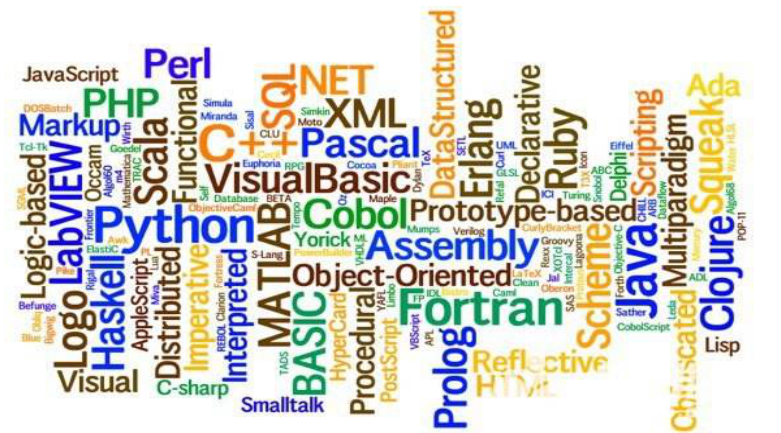
\includegraphics[scale=0.9]{img/C1/1-1/1.png}
	\caption{常见编程语言}
\end{figure}

\section{Hello World!}

\subsection{Hello World!}

\mybox{Hello World!}
\begin{lstlisting}[language=Java]
public class HelloWorld {
    public static void main(String[] args) {
        System.out.println("Hello World!");
    }
}
\end{lstlisting}

\begin{tcolorbox}
	\mybox{运行结果} \\
	Hello World!
\end{tcolorbox}

第一行语句中的public为访问修饰符,一共有三种:public、private、protected。第一行中class表示一个类,类名需要与文件名相同。 \\

第二行中的\lstinline|main()|是程序的入口。 \\

第三行的语句\lstinline|System.out.println()|的作用是在屏幕上输出“Hello World”这个字符串。【;】表示语句结束,注意不要使用中文的分号。

\subsection{字节码文件}

Java编译器(compiler)的作用是将Java源程序编译成中间代码字节码文件。字节码文件是一种和任何具体机器环境及操作系统环境无关的中间代码。Java程序不能直接运行在现有的操作系统,必须运行在Java虚拟机上。Java的特点是一次编写,到处运行。

\newpage

\section{Error or Warning?}

\subsection{Error / Warning}

在编写程序的过程中,错误是不可避免的,错误主要能够分为以下三种类别:

\begin{enumerate}
	\item 语法错误(syntax error):程序的语法不合符编程语言的要求,编译器会反馈报错信息。

	\item 逻辑错误(logical error):人类在编程过程中的逻辑错误,无法被编译器所检测。

	\item 运行时错误(runtime error)例如除以0、数组越界、指针越界、使用已经释放的空间、栈溢出等情况,可以被编译器发现。
\end{enumerate}

\newpage

\section{注释}

\subsection{注释(Comment)}

在编程中加入注释可以增加程序的可读性和可维护性,编译器不会对注释的部分进行编译。 \\

Java中注释分为两类:

\begin{enumerate}
	\item 单行注释:将一行内【//】之后的内容视为注释。
	\item 多行注释:以【/*】开始,【*/】结束,中间的内容视为注释。
\end{enumerate}

\mybox{注释}
\begin{lstlisting}[language=Java]
/*
	这个程序在屏幕上输出Hello World
*/
public class Comment {
	// 主函数
	public static void main(String[] args) {
		System.out.println("Hello World!");		// 输出
	}
}
\end{lstlisting}

\begin{tcolorbox}
	\mybox{运行结果} \\
	Hello World!
\end{tcolorbox}

\newpage

\section{不同语言的Hello World}

\subsection{编程语言对比}

\mybox{C}
\begin{lstlisting}[language=C]
#include <stdio.h>

int main() {
	printf("Hello World\n");
	return 0;
}
\end{lstlisting}

\vspace{0.5cm}
\mybox{C++}
\begin{lstlisting}[language=C++]
#include <iostream>
using namespace std;

int main() {
	cout << "Hello World" << endl;
	return 0;
}
\end{lstlisting}

\vspace{0.5cm}
\mybox{Python}
\begin{lstlisting}[language=Python]
print("Hello World")
\end{lstlisting}

\newpage